% !Mode:: "TeX:UTF-8" 

\chapter{绪论}[Introduction]

\section{课题来源}
本课题来源于深圳市孔雀团队项目子课题,研究的主要内容是使用FPGA对卷积神经网络进行加速从而实现实时的手势识别功能。

\section{课题研究的背景和意义}%[Introduction to the \XeLaTeX way of compiling]
20世纪七八十年代,神经网络\cite{psaltis1988multilayered}的研究在学术界异常火热,尤其是在反向传播算法\cite{rumelhart1986learning}(Backward Propagation)提出以后。但是由于种种因素的限制,如神经网络很难解决训练的问题,当时的计算能力有限等,对神经网络算法研究的热潮很快被SVM,AdaBoost,随机森林等算法取代。直到2012年ImageNet数据比赛中,应用卷积神经网络的AlexNet网络\cite{krizhevsky2012imagenet}一举获得比赛的冠军。AlexNet网络使用五个卷积层、池化层和三个全连接层,最后使用softmax层进行分类。在次之前用以评定分类结果准确性指标Top-5错误率约26\%,而AlexNet的Top-5错误率只有15.3\%。如此大的性能提升,又重新点燃了然就人员对神经网络的研究热情。深度学习的概念来源自人工神经网络,它由Hinton\cite{hinton2006reducing}等人在2006年提出。深度学习中最重要的就是卷积神经网络\cite{bouvrie2006notes}(Convolutional Neural Network,CNN),提出它的最初动机是希望通过建立一种算法,模拟人类大脑分析处理信息的机制,来分析数据,例如语音处理\cite{mikolov2013efficient},图像识别\cite{kavukcuoglu2010learning}。

卷积神经网络的的每层输入是一张图片或若干张特征映射图,将图片或特征映射图与核函数进行卷积,在此过程中能够降低图像的分辨率,摒弃图像中的冗余信息。由于在卷积过程中核函数权值共享,因此使得算法具有一定的位移、缩放和形变抗干扰能力\cite{fukushima1983neocognitron},故此卷积神经网络已经成为图像处理中的一种重要算法。

信息化时代,人与机器,与计算机间的信息交互式是必不可少的。目前最常用的人机交互模式是采用传统的键盘、鼠标和触摸屏等。尽管这些方式已被广泛使用,但是否有更加自然的交互方式,手势识别就是其中一种。使用手势取代传统鼠标键盘,能够使人与机器间的交互更加智能化,简单化。

现场可编程门阵列(Field Programmable Gate Array,FPGA)作为一种半定制电路,既解决了定制电路功能固定,灵活性差的问题,又克服了原有的可编程逻辑器件门电路资源有限的缺陷。此外,现在的一些FPGA都含有ARM颗粒,使得能够从软、硬件方面联合开发。FPGA有大量阵列形式逻辑运算单元,并且在尺寸、功耗以及并行性运算方面有突出的优势,内部丰富的逻辑资源和专用乘法器等可以高度并行的执行运算中大量重复、独立的乘法、加法运算,以较低的功耗实现卷积神经网络的密集运算。
	使用FPGA对加速卷积神经网络的计算主要有如下的优势:
\begin{enumerate}
	\item 成本优势。FPGA能够减少系统部件的总数来降低系统的成本,使其能够适用于需要实时处理图像的产品中。
	\item 速度优势。并行计算的特征能够提供较高的计算性能,起到加速效果。
	\item 功耗降低。FPGA的功耗远远低于CPU和GPU功耗。
	\item 体积更小。FPGA实验平台体积比CPU、GPU小的多,更加适合于嵌入式移动平台应用。
\end{enumerate}

\section{国内外研究现状}
卷积神经网络最大的特征是不需要人为的设计特征分类器,这在一定程度上简化了寻找特征的难题,因为对于一些问题,寻找明显的特征并设计相应的分类器是极其困难的。卷积神经网络以原始数据作为网络的输入,通过大量数据的训练,网络自己学习并优化参数,最终得到特征分类器。但是卷积神经网络也存在计算量大的特征,这使得在以串性运算的计算模式的传统CPU上运算时间长,从而不能满足计算需求\cite{cevher2014convex}。

针对卷积神经网络计算量大的特征,学者研究如何对其进行加速,目前为止采用的加速方案有使用GPU加速,FPGA加速\cite{huang2014}和专用芯片加速。

\subsection{基于GPU的深度学习加速}[Introduction to the application method of the template]
通用处理器(CPU)的内部主要有控制器、寄存器和逻辑单元组成,但是逻辑单元在总体结构中所占的比例较小\cite{shen2007compute},这使得它不适用与卷积神经网络的并行计算。GPU则与之相反,逻辑单元的数量远超过控制器与寄存器的和,它把大规模的数据分解成独立小部分并行执行,使得它的执行效率远远高于CPU。目前主要有NVDIA和AMD两家的GPU,它们的产品如图\ref{nvdiagpu},\ref{amdgpu}所示。

目前,使用GPU对CNN进行加速的技术已经十分成熟并且可取得良好的效果\cite{abdel2012applying}。但随着模型复杂度增加,数据集越来越庞大,单个GPU训练模型也存在性能不足,因此采用多个GPU并行技术训练技术,将模型拆分成小部分分配到多个GPU上存储和训练\cite{wang2017mul}。文献\cite{zhang2013asynchronous}中模型训练使用随机梯度下降算法,并用4块GPU对算法进行加速,最终达到的速度比使用1块CPU训练快3.2倍。在文献\cite{seide20141}中,采用1-bit量化法来减少GPU间数据传输量,降低通信消耗,从而进一步提高网络训练效率,该方法在使用20快GPU训练时达到的效率是1块CPU训练效率的6-7倍。文献\cite{xu2015}将GPU加速与云计算平台相结合,充分利用云计算高效的分布式计算模型和GPU丰富的计算资源,并在此基础上提出一种新型使用大数据计算的并行计算模型。

\begin{figure}[h]
\begin{minipage}{0.5\linewidth}
\centering
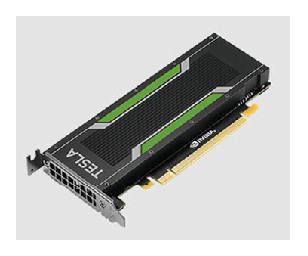
\includegraphics[height = 5cm]{gpu.eps}
\caption{NVIDIA Tesla GPU}
\label{nvdiagpu}
\end{minipage}
\begin{minipage}{0.5\linewidth}
\centering
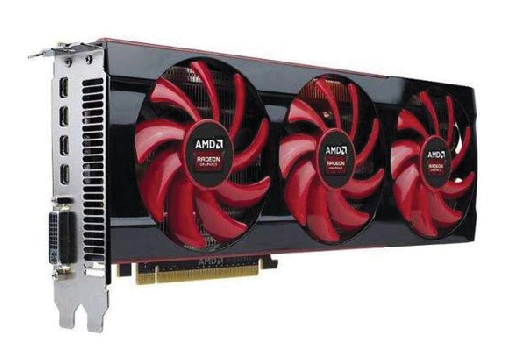
\includegraphics[height = 5cm]{amdgpu.eps}
\caption{AMD Radeon GPU}
\label{amdgpu}
\end{minipage}
\end{figure}

\subsection{基于专用芯片的加速}[Introduction to the application method of the template]

与人工智能常用的几种处理器如CPU(中央处理器)、GPU(图像处理器)相比,专用芯片(Application Specific Integrated Circuit,ASIC)就是针对一些特定应用场景而生,所以在工作效率,性能表现中都更加突出。

在20世纪90年代初,贝尔实验室就开发了能够对卷积神经网络加速的芯片ANNA\cite{boser1991analog}。该芯片包含64个计算单元,能够同时进行64个卷积操作,针对卷积神经网络,该芯片还进行了专门的优化,用4bit来表示其状态值,权重参数使用6bit定点数表示,其峰值运算速度达到约每秒$4x10^{9}$个乘累加操作(Multiply-add Accumulation,MAC)\cite{chen2013,sackinger1992application}。在该芯片上使用卷积神经网路进行手写数字体识别和文本是否有倾斜检测试验时,其展现出的性能要比单独使用DSP计算快10到100倍。相机厂家佳能研发了一款卷积网络芯片,用于低功耗智能相机,完成多类物体的识别,首先在所有位置和规模上使用Gabor滤波器,然后使用简单版本的稀疏和侧向抑制改进,得到最终的模型,并且该模型在功能较少的情况下表现良好\cite{mutch2006multiclass}。文献\cite{desoli201714}中提到一种先进的28nmFD-SOI工艺研制的专用芯片,它有一组支持内核压缩的高效能深度卷积神经网络硬件加速核,片上课重配置数据传输结构,可以用来改善数据重用并减少片上和片外存储器流量,带有外围设备基于ARM的主机子系统和一些高速接口用于图像或其他传感器。Eyeriss芯片\cite{chen2017eyeriss}是由MIT研发的新型芯片,如图\ref{eyeriss}所示,它将数据在处理单元与内存条之间的频率降低,减少在这过程中时间与能量的消耗。与普通GPU相比,Eysriss的每个处理单元都有内存,而不是共享内存,并且它有一个特殊的电路,该电路能够向处理单元分配任务。这些设计使得Eyeriss芯片具有极高的运行效率,其峰值效率能达到手机GPU的10倍。该芯片的其他特性如表\ref{eyerisscharacter}所示。

\begin{table}[h]
\caption{Eyeriss 芯片特性}
\vspace{0.5em}\centering\wuhao
\begin{tabular}{cccc}
	\toprule[1.5pt]
		character & property & character & property\\
	\midrule[1pt]
		Technology & TSMC 65nm LP 1P9M & Core Area & 3.5mm$x$3.5mm\\
		Gate Count & 1852kGates(NAND2) & TOTAL SRAM Size & 181.5KB\\
		On-Chip Buffer & 108KB & \#of PEs & 168\\
		Scratch Pad/PE & 0.5KB & Supply Voltage & 0.82-1.17V\\
		Core Frequency & 100-250MHz & Peak Performance & 16.8-42.0GOPS\\
		Word Bit-width & 16-bit Fixed-Point & Filter Size & 1-32[width] 1-32[height]\\
		\#of Filter & 1024 & \#of Channels & 1-1024\\
		Stride Range & 1-12[horizontal] 1,2,4[vertical] & & \\
	\bottomrule[1.5pt]
\end{tabular}
\label{eyerisscharacter}
\end{table}

\begin{figure}[h]
\begin{minipage}{0.5\linewidth}
\centering
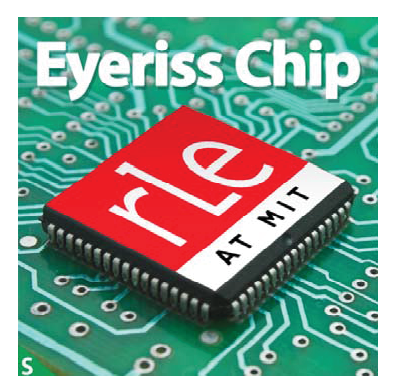
\includegraphics[height = 5cm]{eyeriss.eps}
\caption{MIT Eyeriss Chip}
\label{eyeriss}
\end{minipage}
\begin{minipage}{0.5\linewidth}
\centering
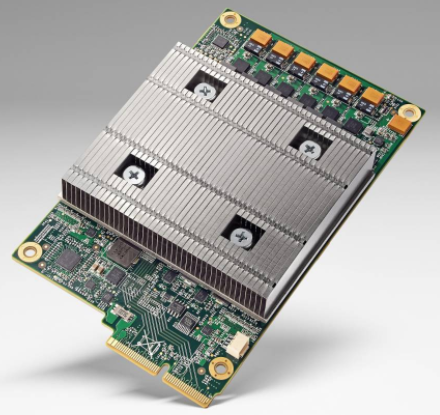
\includegraphics[height = 5cm]{tpu.png}
\caption{Google TPU}
\label{tpu}
\end{minipage}
\end{figure}

2017年体系结构顶会ISCA上,谷歌发布张量处理器(Tensor Processing Unit,TPU)数据中心性能分析论文\cite{jouppi2017datacenter}。TPU,如图\ref{tpu},的核心是65535个8位乘累加矩阵乘法单元和一个28MiB的软件管理的片上内存,矩阵乘法单元的峰值计算能力可达到92TOPS。TPU是基于TensorFlow框架进行神经网络开发的,主要有MLP,CNN和LSTM网络模型。尽管某些应用利用率很低,但TPU平均比快15到30倍,其TOPS/Watt要高出30到80倍。如果在TPU中使用GPU的GDDR5内存,其吞吐量近三倍,并将TOPS/Watt提高到GPU的近70倍和CPU的近200倍。TPU的计算资源主要有矩阵乘法单元,静态存储器SRAM用作缓存,以及硬件连接的激活函数,为了控制这些资源之间的计算,Google还专门为神经网络的推理设计了高级指令。

\subsection{基于FPGA的加速}[Introduction to the application method of the template]

先如今,FPGA芯片都集成了DSP核,提供大量硬件乘累加单元,使得并行的卷积计算成为可能,在FPGA上实现卷积神经网络开始成为一个研究热点。




\subsection{手势识别研究现状}
在学术界,研究人员提出多种算法与方式进行手势识别。在文献\cite{agrawal2011tutor}中,研究人员提出一种识别手势的方法,该方法要求使用者穿戴红色的手套,并且在特征提取时只提取形成手势的红色手套对应的像素区域,如图\ref{gloves}所示。Meenakshi et.al\cite{panwar2011hand}使用RGB图像,它要求使用单一背景图片。由于RGB图对不同光照条件十分敏感,要求先将图片转换到YCbCr空间,随后对其进行二值化并提取相应的手势区域,如图\ref{rgbfinger}所示。

\begin{figure}[h]
\begin{minipage}{0.4\linewidth}
\centering
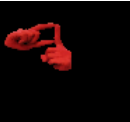
\includegraphics[height = 4cm]{gloves.png}
\caption{Captured with color gloves}
\label{gloves}
\end{minipage}
\begin{minipage}{0.6\linewidth}
\centering
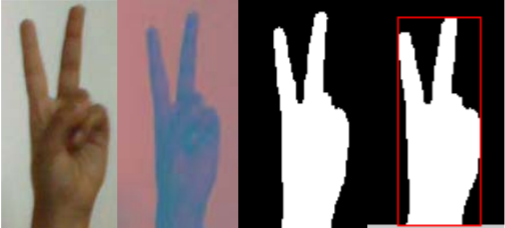
\includegraphics[height = 4cm]{rgbfinger.png}
\caption{RGB image with plain and uniform background}
\label{rgbfinger}
\end{minipage}
\end{figure}



\section{本文的主要研究内容}[Introduction to the application method of the template]

本论文研究了卷积神经网络一般模型的结构特征,在分析网络结构的基础上分析了其在FPGA上实现并行计算的可行性,将整个功能的实现分为PC端训练过程和FPGA端的推理过程。

对于上述的内容,本论文的组织结构如下:

第一章,介绍本论文研究内容的背景和意义,并简单介绍了目前对卷积神经网络的主要加速方案和技术,以及对于手势识别的研究现状,最后概括了本论文的主要研究内容和论文的组织结构;

第二章,介绍卷积神经网络的一般模型;

第三章,
